\documentclass[10pt,a4paper]{article}

\sloppy
\usepackage{caption}
\usepackage{subcaption}
\captionsetup{font = footnotesize, labelfont = bf}
\captionsetup[sub]{font=scriptsize,labelfont= bf}
\setlength{\textwidth}{16cm}
\setlength{\textheight}{23cm}
\addtolength{\hoffset}{-1.5cm}
\addtolength{\voffset}{-1.5cm}
\setlength{\headheight}{35pt}
\usepackage[utf8]{inputenc}
\usepackage[spanish]{babel}
\usepackage{ae}
\usepackage{graphicx}

\usepackage{tikz,pgfplots}
\usepackage{epsfig}
\usepackage{multicol, array}
\decimalpoint
\usepackage{amsmath,amssymb, amsthm}
\usepackage{mathrsfs}
\usepackage{sectsty}
\usepackage{lipsum}
\usepackage{courier}


\usepackage{sectsty}
%\allsectionsfont{\mdseries \raggedright}
\sectionfont{\fontsize{14}{15}\selectfont}
%\chapterfont{\large\sc\centering}
%\chaptertitlefont{\centering}
\subsectionfont{\fontsize{12}{15}\selectfont}
\subsubsectionfont{\fontsize{12}{15}\selectfont}


\usepackage[T1]{fontenc}
\usepackage{textcomp}
\usepackage[slantedGreek]{mathpazo} %% ver psnfss2e
\usepackage{pifont}
\usepackage{newcent}
%\usepackage[small, bf, margin=20pt, tableposition=top]{caption}

\usepackage{fancyhdr}


\setlength{\parskip}{2mm}



\theoremstyle{definition}
\newtheorem{example}{Ejercicio N$^o$}

\pagestyle{fancy}
\headheight = 25pt 
\lhead{Mecánica del Continuo 2021 -  U.N.S.L. \\ Depto. de Física -  Licenciatura en Física}
\rhead{
\includegraphics[width=1cm]{/home/juan/Documentos/Docencia/unsl.jpg}}
\vspace*{0.25cm}


\begin{document}



\begin{center}
{\bf \large Mecánica del continuo \\ Consulta Trabajo Práctico N$^o 2:$ }
\end{center}

\medskip

%EJERCICIO5

\section*{Ejercicio 1}
Considerar el movimiento descripto por:


\begin{equation}\label{e1}
x_1 = kt+X_1 ; \quad x_2 = X_2 ;\quad x_3 = X_3
\end{equation}
\noindent donde la coordenada material especifica la posici\'on de la part\'icula a $t=0$.

\begin{itemize}
\item[a)] Determine la velocidad y aceleraci\'on de la part\'icula en la descripción material. Obtenga la trayectoria de las partículas cuyas coordenadas materiales están dadas por $X_1 = 0 m\, , X_2 \, , X_3 $
\item[b)] Determine los campos de velocidad y aceleración (descripción espacial). Grafique utilizando \textit{Mathematica} para $t = 0 \, s$ y para $t = 100 \, s$. 
\item[c)] Encuentre la razón temporal de cambio de la temperatura que experimenta una partícula, siendo que el campo de temperatura está especificado por $\Theta(x)=A x_1$. 
\end{itemize}

\begin{center}------------------------------------------------------------------------------\end{center}

\subsection*{Solución}

\textbf{a)}
 Para determinar la velocidad y la aceleración de la partícula en la descripción material, es importante que miremos la ec. 3.4.2 del \textit{Lai, Introduction to Continuum Mechanics (4ta Ed.)}. Ahí se lee que:

\begin{equation} \label{evel}
\mathbf{v} = \Big( \frac{\partial \mathbf{x}}{\partial t} \Big)_{X_i fixed} \equiv \frac{D \, \mathbf{v}}{D \, t}
\end{equation}

Si aplciamos la ec. anterior a las ecs. \eqref{e1}, tenemos:

\begin{equation}\label{e1vs}
v_1 = k \quad v_2 = v_3 = 0
\end{equation}

\noindent donde en las ecs. \eqref{e1vs} tenemos que todas las partículas tienen una velocidad costante $v_a = k$.

Si aplicamos la ec. de la aceleración de una partícula, tenemos:
\begin{equation}\label{ea1}
\mathbf{a} = \frac{\partial \mathbf{v}}{\partial t} + \Big(  \mathbf{\nabla v} \Big) \mathbf{v}
\end{equation}

\noindent en la ec. \eqref{ea1} tenemos que $\mathbf{v} \neq \mathbf{v}(t)$, con lo que el primer término del lado derecho de la ec.\eqref{ea1} es $\partial \mathbf{v} / dt = 0$. El segundo término tiene el campo tensorial que es el \textit{gradiente del campo de velocidades}. Como el campo de velocidades no tiene dependencia espacial alguna, ergo, $\nabla \mathbf{v}\mathbf{v} = 0$. El campo de aceleración es $\mathbf{a} = 0$.

Con respecto al conjunto de partículas (que es un conjunto infinito no denumerable)  $(0,X_2,X_3)$, vemos que las velocidadesestán en la dirección $\mathbf{e_1}$, a velocidad constante, con lo cual su aburrida trayectoria será estár en $(X_1 = 0,X_2,X_3)$ a $t = 0$, y en general tendremos $(kt, X_2,X_3)$.


\pagebreak

\textbf{b)}

Los campos de velocidad y aceleración son bastante aburridos también en la descripción espacial. Como $\mathbf{v} = k \mathbf{e_1}'\; \forall \mathbf{X}$, entonces la descripción espacial tendrá la misma velocidad en cualquier punto del espacio $\mathbf{x}$ (si nos paramos en $\mathbf{x}$ vemos pasar todas las partículas con la misma velocidad, ergo, la aceleración en la descripción espacial también es $\mathbf{a} = \mathbf{0}$.

\textbf{c)}

El campo de temperatura aumenta con la coordenada espacial $x_1$, con una funcionalidad simple $\Theta  = Ax_1$. Tenemos entonces:

\begin{equation}
\frac{D \Theta}{D t} = \overbrace{\frac{\partial \Theta}{\partial t}}^0 + \frac{\partial \Theta}{\partial x_i} \frac{\partial x_i}{\partial t} = \frac{\partial \Theta}{\partial x_i} \frac{\partial x_i}{\partial t} = A k 
\end{equation}

\noindent con lo cual podemos vislubrar que, si el campo de temperatura tiene una tasa de aumento $A$ respecto de la coordenada $x_1$ y las partículas viajan aumentando esa coordenada en el tiempo a una tasa (velocidad) $k$, entonces la temperatura de una partícula aumenta a una tasa $Ak$, lo cual no es loco.



\section*{Consulta Ejercicio 5}
Considere el continuo cuyo campo de velocidad viene dado por:

\begin{equation} \nonumber
v_i=\dfrac{x_i}{1+t}
\end{equation}
\noindent Encuentre la ecuaci\'on de movimiento y el campo\footnote{Esta palabra está mal aquí, cuando hablamos de campo en general pensamos en una representación espacial, y lo que pide a continuación es la descripción material...} de aceleraci\'on en la descripci\'on material.

 ----------------------------------------------------------------------
 
Bueno, acá va prolijo. Recuerdo de notación:  Minúsculas, escalares. Mayúsculas, tensores (salvo coordenadas materiales). Negritas, vectores. 
\vspace{1cm}
a) Ecuaciones de movimiento:

Como ya sabemos, las ecuaciones de movimiento son $x_i = f(\mathbf{X}, t)$

La velocidad está en la descripción espacial, es decir,  $v_i(x_i, t)$. Concretamente:

\begin{equation}\label{ev}
v_i =\dfrac{x_i}{1+t}
\end{equation}

\noindent ojo que la ec. anterior no tiene como definición la definición de velocidad. La función $v_i(x_i, t)$ describe el cambio de velocidades de las partículas \textit{que pasan} por un punto fijo $x_i$ en un marco de referencia, y no el cambio en la posición respecto del tiempo de \textbf{una} partícula.

Entonces, en la ec.(\ref{ev}) hacemos:

\begin{equation}\label{eint}
\dfrac{\partial x_i}{\partial t} =\dfrac{x_i}{1+t} \Rightarrow \int_{x_i = X_i}^{x_i} \dfrac{dx_i}{x_i} = \int_{t = 0}^{t} \dfrac{dt}{1+t}
\end{equation}


La solución a la ec.(\ref{eint}) queda:

\begin{equation} \label{esol}
ln(\dfrac{x_i}{X_i}) = ln(1+t) \Rightarrow x_i(X_i, t)  = X_i \; (1+t) + g(X_{j \neq i})
\end{equation}

\noindent si miramos la ec.(\ref{esol}) se nota que agregamos una función no especificada $g(X_j)$, para tener en cuenta que estamos integrando una ec. a derivadas parciales. La función $g(X_{j\neq i})$ es una función arbitraria de las coordenadas materiales...que no vamos a usar...pero que sería muy simple de calcular...¿cómo? Tarea pa las casas.

El resultado que nos da para las ecs. de movimiento es entonces:

\begin{eqnarray}
\label{e51} x_1(X_1, t)  = X_1 \; (1+t) \\
\label{e52} x_2(X_2, t)  = X_2 \; (1+t) \\
\label{e53} x_3(X_3, t)  = X_3 \; (1+t) \
\end{eqnarray}


\textbf{b)} ...calcular la aceleración en la descripción material, es decir, la tasa de cambio temporal en las velocidades de cada partícula.

Esto es, de la ecs.(\ref{e51}, \ref{e52}, e53) hacemos:

\begin{equation} \label{eacel}
a_i(\mathbf{X}, t) = \dfrac{\partial^2 x_i(\mathbf{X}, t)}{\partial t^2}
\end{equation}

Lo que nos deja:

\begin{equation}
a_i = 0 \; \forall i= 1,2,3
\end{equation}


Entonces, las partículas no experimentan aceleración a pesar de que la velocidad en un punto del campo cambia en el tiempo.

\line(1,0){100}

\line(1,0){180}


%EJERCICIO6

\section*{Consulta Ejercicio 6}
Dado el campo de velocidad:

\begin{equation}\label{ee6}
 v_1=-2x_2 \; \; \; v_2=2x_1
\end{equation}
\begin{itemize}
\item[a)] Encuentre el campo de aceleraci\'on.
\item[b)] Obtenga la expresi\'on de la linea de camino (``pathline'') del continuo. 
\item[c)] Grafique el campo de aceleración en la descripción espacial.
\end{itemize}

%\line(1,0){100}
\textbf{a)} Encontrar el campo de aceleración es simple, ya que contamos con la ecuación del Lai, 4$^{ta}$ ed. que dice:


\begin{equation}\label{ealai}
\mathbf{a} = \dfrac{\partial \mathbf{v}}{\partial t} + \nabla \mathbf{v} \; \mathbf{v}
\end{equation}

Podemos calcular, usando las ecs.(\ref{ee6}), las funciones que posee la expresión (\ref{ealai}), con lo que el primer término queda:

\begin{equation}
\dfrac{\partial \mathbf{v}}{\partial t} = \mathbf{0}
\end{equation}

\noindent es decir, la velocidad en un punto (descripción espacial) no cambia con el tiempo. Sólo depende de las coordenadas espaciales.

El segundo término de la ec.(\ref{ealai}) queda:

\begin{eqnarray}
\nonumber
\nabla \mathbf{v} \; \mathbf{v}  = &    
\begin{pmatrix}
\partial v_1 / \partial x_1 &  \partial v_1 / \partial x_2 & \partial v_1 / \partial x_3\\ 
\partial v_2 / \partial x_1 &  \partial v_2 / \partial x_2 & \partial v_2 / \partial x_3\\ 
\partial v_3 / \partial x_1 &  \partial v_3 / \partial x_2 & \partial v_3 / \partial x_3\\ 
\end{pmatrix}
\begin{pmatrix}
v_1 \\
v_2 \\
v_3 \\
\end{pmatrix}
\Rightarrow & \\ 
\nabla \mathbf{v} \; \mathbf{v}  = &  
\begin{pmatrix}
0 &  -2 & 0 \\ 
2 &  0 & 0 \\ 
0 &  0 & 0 \\ 
\end{pmatrix}
\begin{pmatrix}
-2 x_2 \\
2 x_1 \\
0 \\
\end{pmatrix}
= & 
\Big( -4x_1 \; \; -4x_2 \; \; 0 \Big)
\end{eqnarray}

\noindent juntando lo anterior, tenemos que la aceleración en la descripción espacial (el \textit{campo} de aceleración) es:

\begin{equation} \label{e6ae}
\mathbf{a}(x_1,x_2) = -4 x_1 \mathbf{e_1} - 4x_2 \, \mathbf{e_2}  
\end{equation}

\noindent una cosa interesante del campo de velocidades y el de aceleración, dado por la ec.(\ref{e6ae}) es que:


\begin{equation}\nonumber
\mathbf{v} \cdot \mathbf{a} = \Big(-2x_2\, \mathbf{e_1} + 2x_1 \, \mathbf{e_2} \Big) \cdot \Big(-4 x_1 \mathbf{e_1} - 4x_2 \, \mathbf{e_2}\Big) = \mathbf{0}
\end{equation}

\noindent lo anterior nos da una idea de movimiento circular, ¿no?, la aceleración perpendicular a la velocidad para cualquier tiempo y para cualquier coordenada...


--------------------------------


\textbf{b)} Encontrar la trayectoria o \textit{pathline}

Las trayectorias son, simplemente...las trayectorias\footnote{El conjunto de puntos $x_1, x_2, x_3$ que conforman las posiciones de una partícula para cierto intervalo de tiempo.}, y están definidas por la ecuación de movimiento $\mathbf{x}(\mathbf{X}, t)$. Sin embargo, a veces es posible deshacerse del parámetro del tiempo, combinando las ecuaciones.

A veces simple, otras no tanto, en este caso:


\begin{eqnarray}
\label{e61} v_1 = \dfrac{\partial x_1}{\partial t}  = -2 x_2  \\
\label{e62}v_2 = \dfrac{\partial x_2}{\partial t} = 2 x_1 \
\end{eqnarray}




\noindent derivando respecto del tiempo las ecs. anteriores, tenemos:
\begin{eqnarray}
\label{e61s}\dfrac{\partial^2 x_1}{\partial t^2}  = -2 \dfrac{\partial x_2}{\partial t} = -4x_1 \\
\label{e62s}\dfrac{\partial^2 x_2}{\partial t^2}  = 2 \dfrac{\partial x_1}{\partial t} = -4x_2 \\
\end{eqnarray}

\noindent las ecs.(\ref{e61s} y \ref{e62s}) pueden integrarse dos veces para dar:

\begin{eqnarray}
\label{e61ss}x_1 = r\; cos(2t) \\
\label{e62ss}x_2 = r\; sin(2t) \\
\end{eqnarray}

\noindent donde $r = \sqrt{X_1^2 + X_2^2}$ es la constante de integración de las ecs(\ref{e61s} y \ref{e62s}). Nos salteamos algunos pasos, pero si derivamos dos veces las ecs.(\ref{e61ss} y \ref{e62ss}), se puede ver que obtenemos las velocidades y las aceleraciones que calculamos. 

Dicho lo anterior, queda saber que las ecs.(\ref{e61ss} y \ref{e62ss}) nos dicen explicitamente que esto que teníamos entre manos es un movimiento circular...de hecho, podemos sacar el pathline y deshacernos del tiempo, usando la identidad trigonométrica fundamental:

\begin{equation}
x_1^2 + x_2^2 = r^2 \equiv constante \label{e63sol}
\end{equation}

\noindent con todo este complicado proceso, tenemos el \textit{pathline} o \textit{trayectoria} de la partícula es un círculo cerrado.

\line(1,0){100}

\textbf{c)} Graficar el campo de aceleración es simple con Mathematica. No hay que perder de vista que un campo vectorial se grafica habitualmente con vectorcitos en una red definida de puntos. Lo podemos hacer con el comando:

\noindent \texttt{StreamDensityPlot[\{\{-4 x, -4 y\}, div[x, y]\}, \{x, -5, 5\}, \{y, -5, 5\}, \linebreak
 ColorFunction -> ''RedBlueTones´´, StreamStyle -> Black,  \linebreak
 StreamPoints -> Medium, ImageSize -> Large]\}}



\begin{figure}[h!]
\begin{subfigure}{.50\textwidth}
  \centering
 \title{Gráfico de Contorno de $\chi^2$}  
  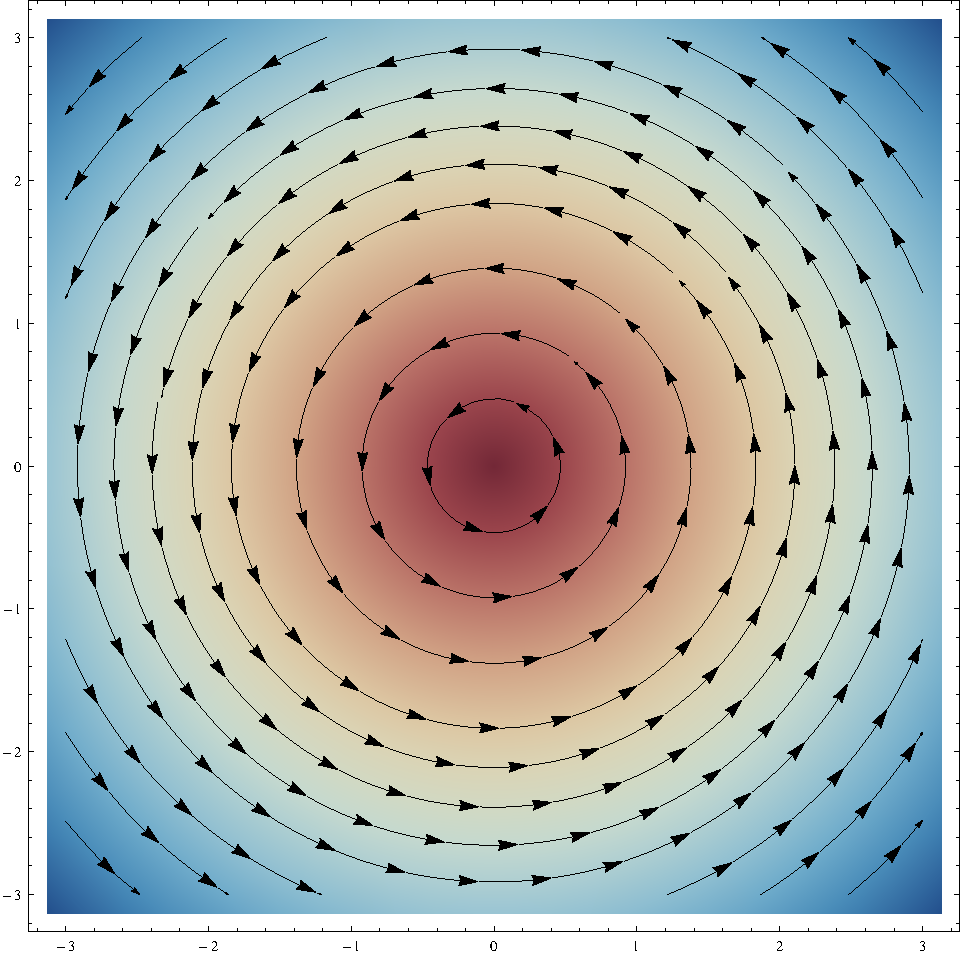
\includegraphics[width=1\linewidth]{vel6.pdf}
  \caption{Velocidad, Descripción espacial.}
  \label{gconto}
\end{subfigure}%
\begin{subfigure}{.50\textwidth}
\title{} 
  \centering
   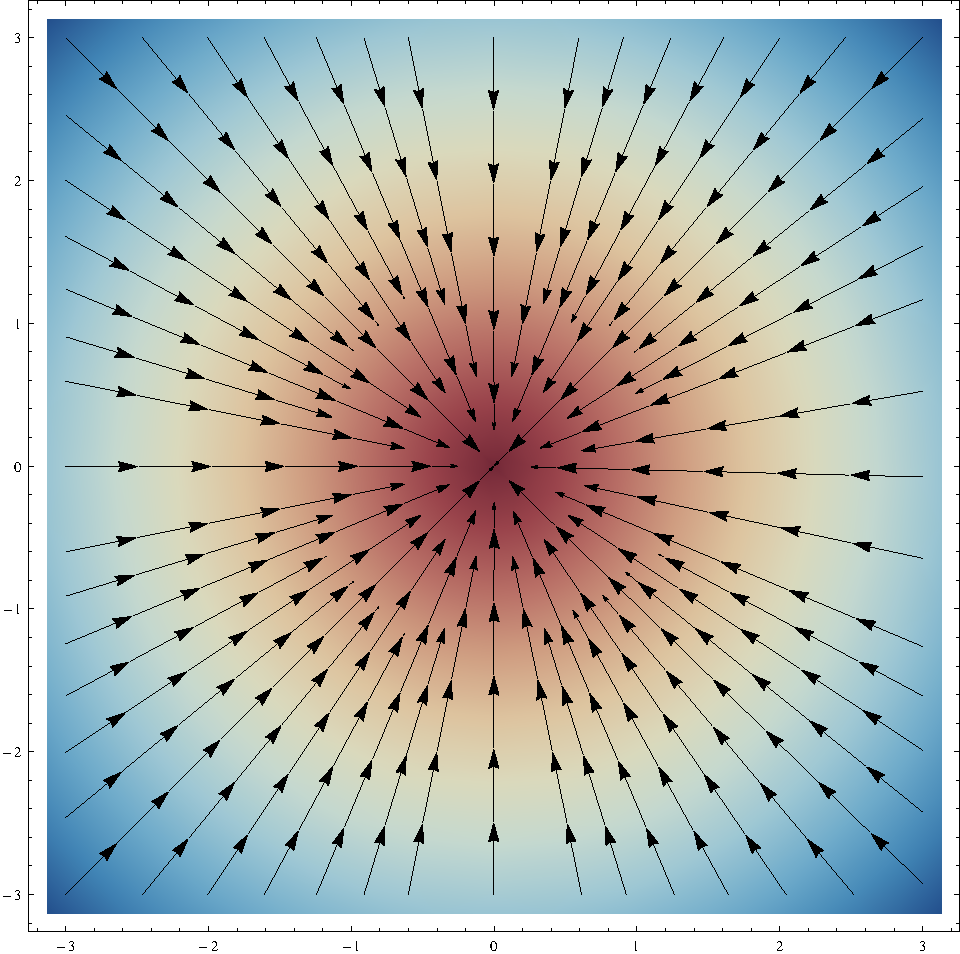
\includegraphics[width=1\linewidth]{acel6.pdf}
  \caption{Campo de aceleración.}
  \label{gtresd}
\end{subfigure}
\caption{Los colores representan la divergencia del campo  (y no se los pude sacar fácilmente!). Sin embargo se ve bonito...es importante notar que es de hecho un campo que se mueve de manera circular en torno a $\mathbf{x = \mathbf{0}}$.}
\end{figure}


%EJERCICIO7
\section{Consulta Ejercicio 7}

En la descripci\'on espacial, la ecuaci\'on para evaluar la aceleraci\'on es:
\begin{align*}
\dfrac{Dv}{Dt}=\left(\dfrac{\partial \mathbf{v}}{\partial t} \right)_x + (\nabla \mathbf{v}) \mathbf{v}
\end{align*}
\noindent Esta ecuación es no-lineal, es decir si consideramos dos campos de velocidad $v^A, \: v^B$, se cumple que:
\begin{align*}
a^A+a^B \neq a^{A+B} 
\end{align*}
\noindent donde $a^A$ y $a^B$ son los campos de aceleración de los campos de velocidad $v^A$ y $v^B$ (respectivamente) y $a^{A+B}$ es el campo de aceleración del campo de velocidad $v=v^A+v^B$.

Suponga un campo bidimensional dado por:

\begin{flalign*}
& v^A=-2x_2e_1+2x_1e_2 \\
& v^B=2x_2e_1-2x_1e_2 
\end{flalign*}

\begin{itemize}
\item[a)] Verifique esta desigualdad para los campos de velocidad anterior. Grafique $a^{A+B}$
\item[b)] Obtenga la suma $a^A + a^B$. Grafíquela.
\item[c)] ¿Qué condición debería cumplir $\nabla \mathbf{v}$ para que las gráficas anteriores coincidan?
\end{itemize}


\line(1,0){100}

\line(1,0){180}

Solución

\textbf{a)} Verifique esta desigualdad para los campos de velocidad anterior. Grafique $a^{A+B}$

Hacemos la suma de las velocidades:

\begin{equation}\label{e71}
v^{A + B} = v^A + v^B = \mathbf{0}
\end{equation}

\noindent de paso nos fijamos que las expresiones de $v^A$ y $v^B$ son igualitas a las rotaciones del Ej. 6, sólo que contrapuestas (una va en el sentido de las agujas del relós y la otra en sentido inverso).

Entonces si planteamos la aceleración material a partir del campo de velocidades de la ec.(\ref{e71}) obviamente nos da $\mathbf{0}$.

---------------------------------------------------------------
\vspace{1cm}

\textbf{b)} Obtenga la suma $a^A + a^B$. Grafíquela.

Aplicamos la ec.(\ref{eacel}) reemplazando las expresiones de $v^A$ y $v^B$:

\begin{eqnarray}
a^A & = &-4x_1\mathbf{e_1} - 4x_2\mathbf{e_2} \label{aA}\\
a^B & = &-4x_1\mathbf{e_1} - 4x_2\mathbf{e_2} \label{aB} \
\end{eqnarray}

\noindent las aceleraciones son igualitas...qué cosa esto del continuo que a partir de campos de aceleración iguales salen rotaciones opuestas (la info de para qué lado rota puede ser encontrada en $\nabla \mathbf{v})$, y en otras cuentas, antes que en el campo de aceleración.

Si las sumamos tenemos:
\begin{equation}
a^A + a^B = -8x_1\mathbf{e_1} + -8x_2\mathbf{e_2} \label{easum}
\end{equation}

\noindent lo que nos deja un campo de aceleración con la misma pinta en el del Ejercicio 6.

\begin{figure}[h!]
\centering
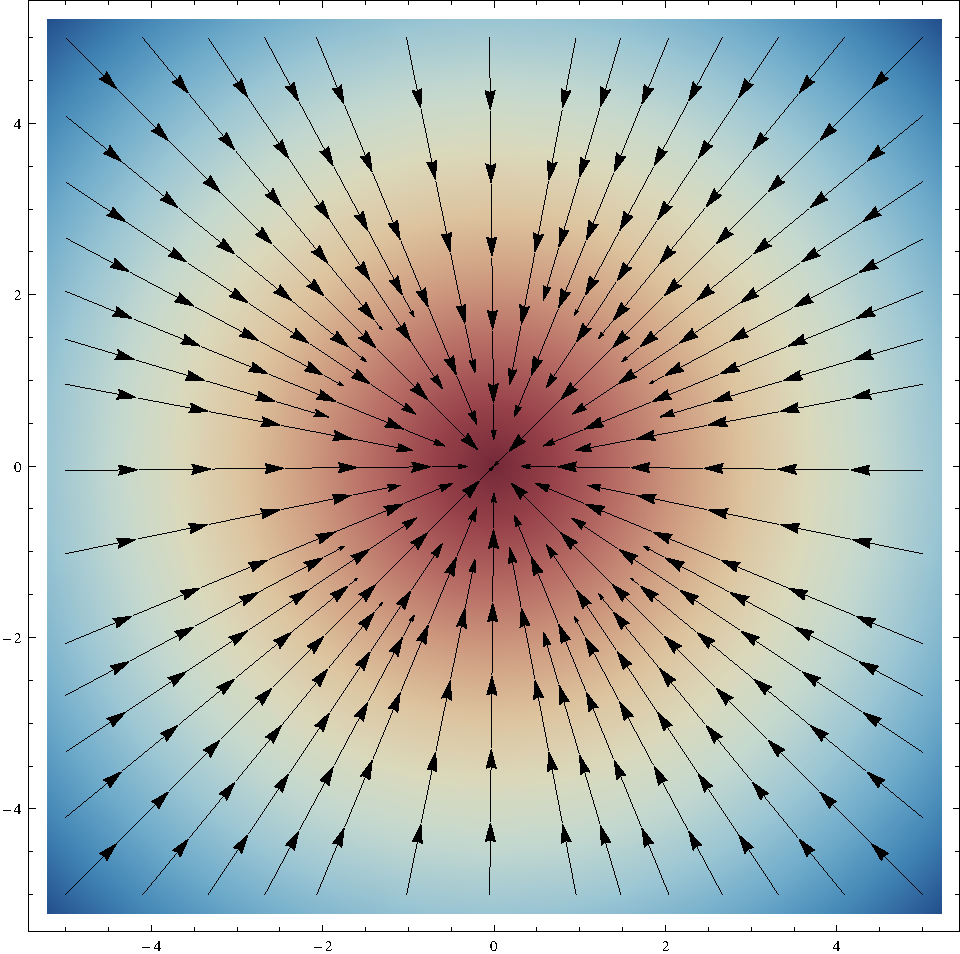
\includegraphics[width=0.5\linewidth]{acel7aplusb.pdf}
  \caption{Aceleración $a = a^A + a^B$, nada tiene que ver con el $\mathbf{a} = \mathbf{0}$ que obtuvimos antes...}
  \label{gae7}
\end{figure}


\noindent con esto concluímos...


---------------------------------------------------------------
\vspace{1cm}

\textbf{c)} ¿Qué condición debería cumplir $\nabla \mathbf{v}$ para que las gráficas anteriores coincidan?

Más fácil, imposible (mentira, estuve un rato largo pensando).

Sean:
\begin{eqnarray}
a^A = \dfrac{Dv^A}{Dt} & = & \dfrac{\partial v^A}{\partial t} + (\nabla v^A) \, v^A  \nonumber \\
a^B = \dfrac{Dv^B}{Dt} & = & \dfrac{\partial v^B}{\partial t} + (\nabla v^B) \, v^B  \nonumber \\
a^A + a^B & = & \dfrac{\partial (v^A + v^B)}{\partial t} + (\nabla v^A) \, v^A + (\nabla v^B) \, v^B \label{e73c3}
\end{eqnarray}

y sea:
\begin{equation}
a^{A + B}  = \dfrac{D(v^A + v^B)}{Dt} = \dfrac{\partial (v^A + v^B)}{\partial t} + (\nabla v^A) \, v^A + (\nabla v^B) \, v^B + \Bigg[ (\nabla v^A) \, v^B + (\nabla v^B) \, v^A \Bigg]\label{e7c4}
\end{equation}

\noindent así, comparando la ec.(\ref{e73c3}) con la ec.(\ref{e7c4}), tenemos que la cantidad entre corchetes debe ser $\mathbf{0}$. Así:
\begin{equation}
 (\nabla v^A) \, v^B + (\nabla v^B) \, v^A = 0 \label{finalfin}
\end{equation}

para que la ec.(\ref{finalfin}) sea $\mathbf{0}$, la opción menos restrictiva sobre los campos $v^A$ y $v^B$ es que no dependan de las coordenadas espaciales, y sólo de la coordenada temporal, es decir, campos constantes en el espacio es lo único\footnote{No es lo punico, pero dudo que algo sobreviva a la carnicería de funciones al desarrollar todo el gradiente y los productos...} que nos puede asegurar que $a^{A+B} = a^A + a^B$.


\end{document} 